The quality control and quality assurance procedures for the individual components of the ProtoDUNE-SP detector are collected in this chapter.

%%%%%%%%%%%%%%%%%%%%%%%%
\section{APA}

Each ProtoDUNE-SP APA will be subject to a testing program during production that will demonstrate their compliance with the design and manufacturing requirements for the experiment.  Given the large size of the APAs, and the highly specialized cryogenic and electronic infrastructure necessary for their designed operation, the testing plan followed during production is necessarily targeted at those features of the APAs which can be addressed prior to final installation in the cryostat.  A separate suite of testing, in a cryogenic environment, is planned to be conducted at CERN, as described in ???? \fixme{is there a section in the TDR for this cold-box test?}.

The tests described in this section will be conducted on APAs during construction, as well as on completed APAs.  Subcomponents ($e.g.$ - wire boards, BeCu wire, etc..) are verified or tested by the appropriate vendor or subsystem manager prior to their use in APA construction.  Each APA will be subject to the testing listed in Table \ref{tab:apatesting}.   Many of the tests (e.g. - tension, continuity, isolation, position survey, bias voltage) are repeated as each successive wire layer of the APA is added, testing the newly installed wires as well as spot-checking wires from previously installed layers. The summary of the tests on each APA, and the associated data collecting during the tests, are recorded in a traveler.

\begin{cdrtable}[APA Testing]{llr}{apatesting}{Tests to be conducted on APAs during production.}
Label & Requirement & Test Method  \\ \toprowrule
Tension      & All wires must be tensioned to 5$\pm$1 N & Laser Survey \\ \colhline
Cryo       &  All APA must operate at 87 K  & Cryotest \\ \colhline
Electrical       & All wires electrically connected at top/bottom of APA  & Continuity \\ \colhline
Isolation & Neighboring APA wires have $\geq$1 M$\Omega$ resistance & Multimeter\\ \colhline
Voltage & Anode planes must hold $\geq$100$\%$ bias & Bias \\ \colhline
Position & All wires must be within 500 $\mu$m of design location & Survey\\ \colhline
Frame & APA frame satisfies all bow/twist/fold criteria & Survey\\ \colhline
\end{cdrtable}

%%%%%%%%%%%%%%%%%%%%%%%%
\section{CPA}

The following activities are planned to assure the CPA meets all design requirements as defined in the fabrication drawings and description in the sections above:
\begin{itemize}
\item Performed 35 ton HV test at FNAL.
\item Fabricate four prototype CPAs to test the design and fabrication and assembly methods.
\item Installation test at Ash River:
\begin{itemize}
\item Test the lifting and handling of the four prototype CPA's.
\item  Load the 4 prototype CPA's with FC modules and test and evaluate their installation.
\end{itemize}
\item Develop a QC plan for inspecting every fabricated part of the CPA frame to make sure they meet the dimensions and tolerances on the fabrication drawings.
\item Develop a QC plan for inspecting and measuring each CPA module and completed CPA plane to ensure they meet the dimensions and tolerances on the drawings.
\item Perform tests of each joint in the CPA frame (see Section 3) to ensure that their design and strength meets the load requirements.
\item Create an integrated model of the entire TPC to evaluate interfaces and installation methods.  
\item Develop a QC for receiving the resistive panels.  Measure the dimensions to confirm they meet the drawings and setup a plan and acceptance criteria to insure that panel resistance is acceptable.
\item Develop a QC  HV test at CERN for evaluating side to side and top to bottom resistance for each completed CPA but after final assembly and after hanging during installation.  
\end{itemize}

%%%%%%%%%%%%%%%%%%%%%%%%%
\section{FC}

The following activities are/will be performed to assure the field cage meets all design criteria as defined in the fabrication drawings and description in the sections above:
\begin{itemize}
\item	Fabricate prototype FCs to test the design and fabrication and assembly methods.
\item	Installation test at Ash River:
\begin{itemize}
\item	Test the lifting and handling of the prototype FCs.
\item	Mount the prototype FCs to the CPA modules and test and evaluate their installation.
\end{itemize}
\item	Develop a QC plan for inspecting every fabricated part of the FC frame to make sure they meet the dimensions and tolerances on the fabrication drawings.
\item	Develop a QC plan for inspecting and measuring each FC module and completed FC plane to insure they meet the dimensions and tolerances on the drawings.
\item	Perform tests of each joint in the FC frame (see Section XX) to insure that their design and strength meets the load requirements.
\item	Create an integrated model of the entire TPC to evaluate interfaces and installation methods.  
\end{itemize}

 %%%%%%%%%%%%%%%%%%%%%%%%%
\section{HV}

\fixme{no info contributed}

  %%%%%%%%%%%%%%%%%%%%%%%%%
\section{PDS}

\fixme{no info contributed}

%%%%%%%%%%%%%%%%%%%%%%%%%
\section{CE}

A full description of the testing procedures is being developed in a separate document. A 
summary is provided here.

%%%%%%%%%%%%%%%%%%%%%%%%%
\section{DAQ}

The DAQ for ProtoDUNE-SP does not require large numbers of custom hardware components to 
be built and tested.  There will be 8 COBs with 8 RCEs each, 2 FELIX cards, 24 SSPs, the timing 
and trigger systems and off-the-shelf hardware (computers, network switches, storage, etc.).
As such, a significant amount of automation is not needed to test and qualify the 
components.  

Qualification tests of the RCEs, FELIX boards, SSPs, timing and trigger systems will
be driven by the host institutes producing those systems.  Reception tests will be 
performed to identify any failures due to transport.  In order to fully qualify the 
boards, they will need to be individually tested with control samples.  Data generators
will be used in place of the front-end electronics where applicable.  Full data rate 
testing will be performed when the first full detector slice is in place at EHN1 (expected
Q2 2017).  Data challenges will take place during Q1 2017 in advance of the arrival of the 
first APA, and again as the computing system expands to its full capacity.

%%%%%%%%%%%%%%%%
\subsection{Prototype testing}
\label{subsubsec:ce_install_proto}

Dedicated test boards for the FE ASIC and ADC ASIC,
were used to characterize the performance of prototype ASICs at both 300~K and 77~K,
and taking them through multiple thermal cycles.
An automated test board was built for the FE ASIC (Fig.~\ref{fig:tpcce_FE_TestBoard})
to evaluate large numbers of FE ASICs at room temperature,
and another such board is currently being designed for the ADC ASIC (Fig.~\ref{fig:tpcce_ADC_TestBoard}).

\begin{cdrfigure}[FE ASIC testboard]{tpcce_FE_TestBoard}{FE ASIC testboard.}
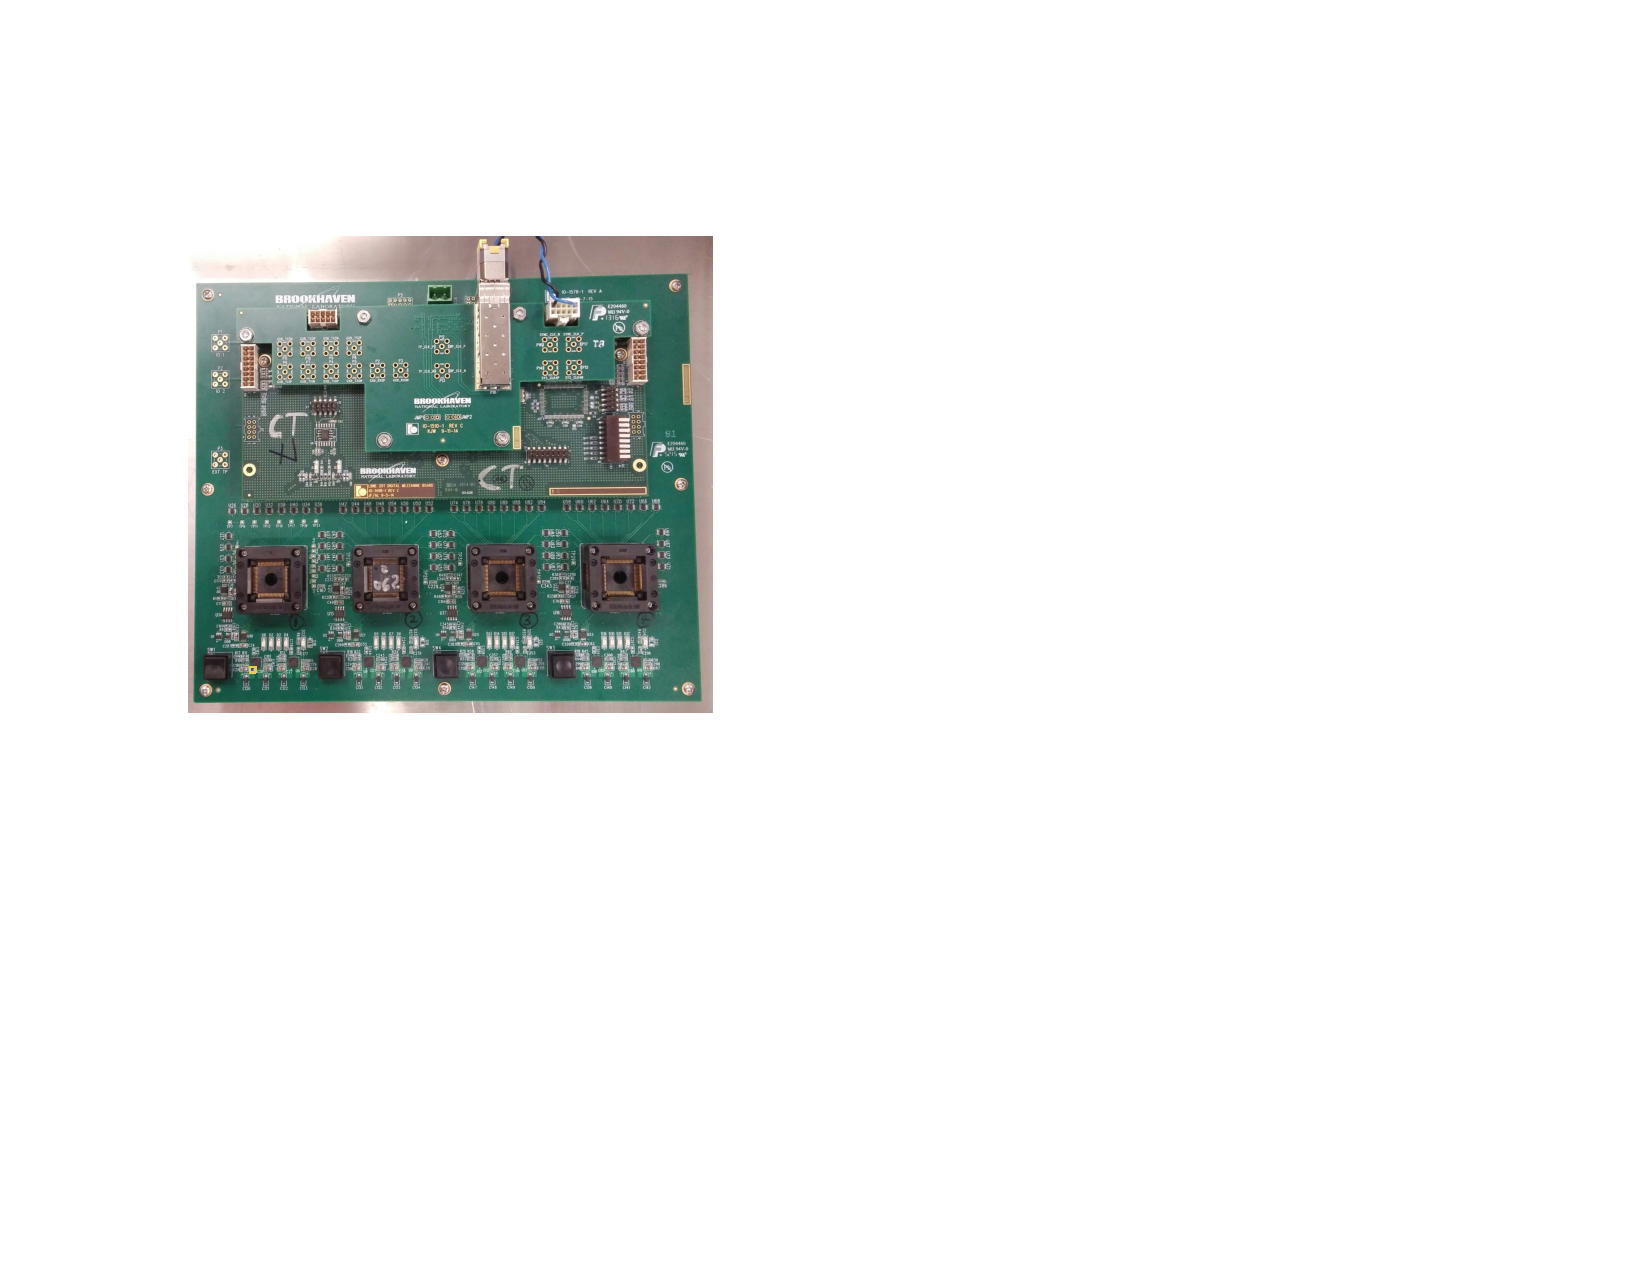
\includegraphics[width=0.6\linewidth]{tpcce_FE_TestBoard.pdf}
\end{cdrfigure}
\begin{cdrfigure}[ADC ASIC testboard]{tpcce_ADC_TestBoard}{ADC ASIC testboard.}
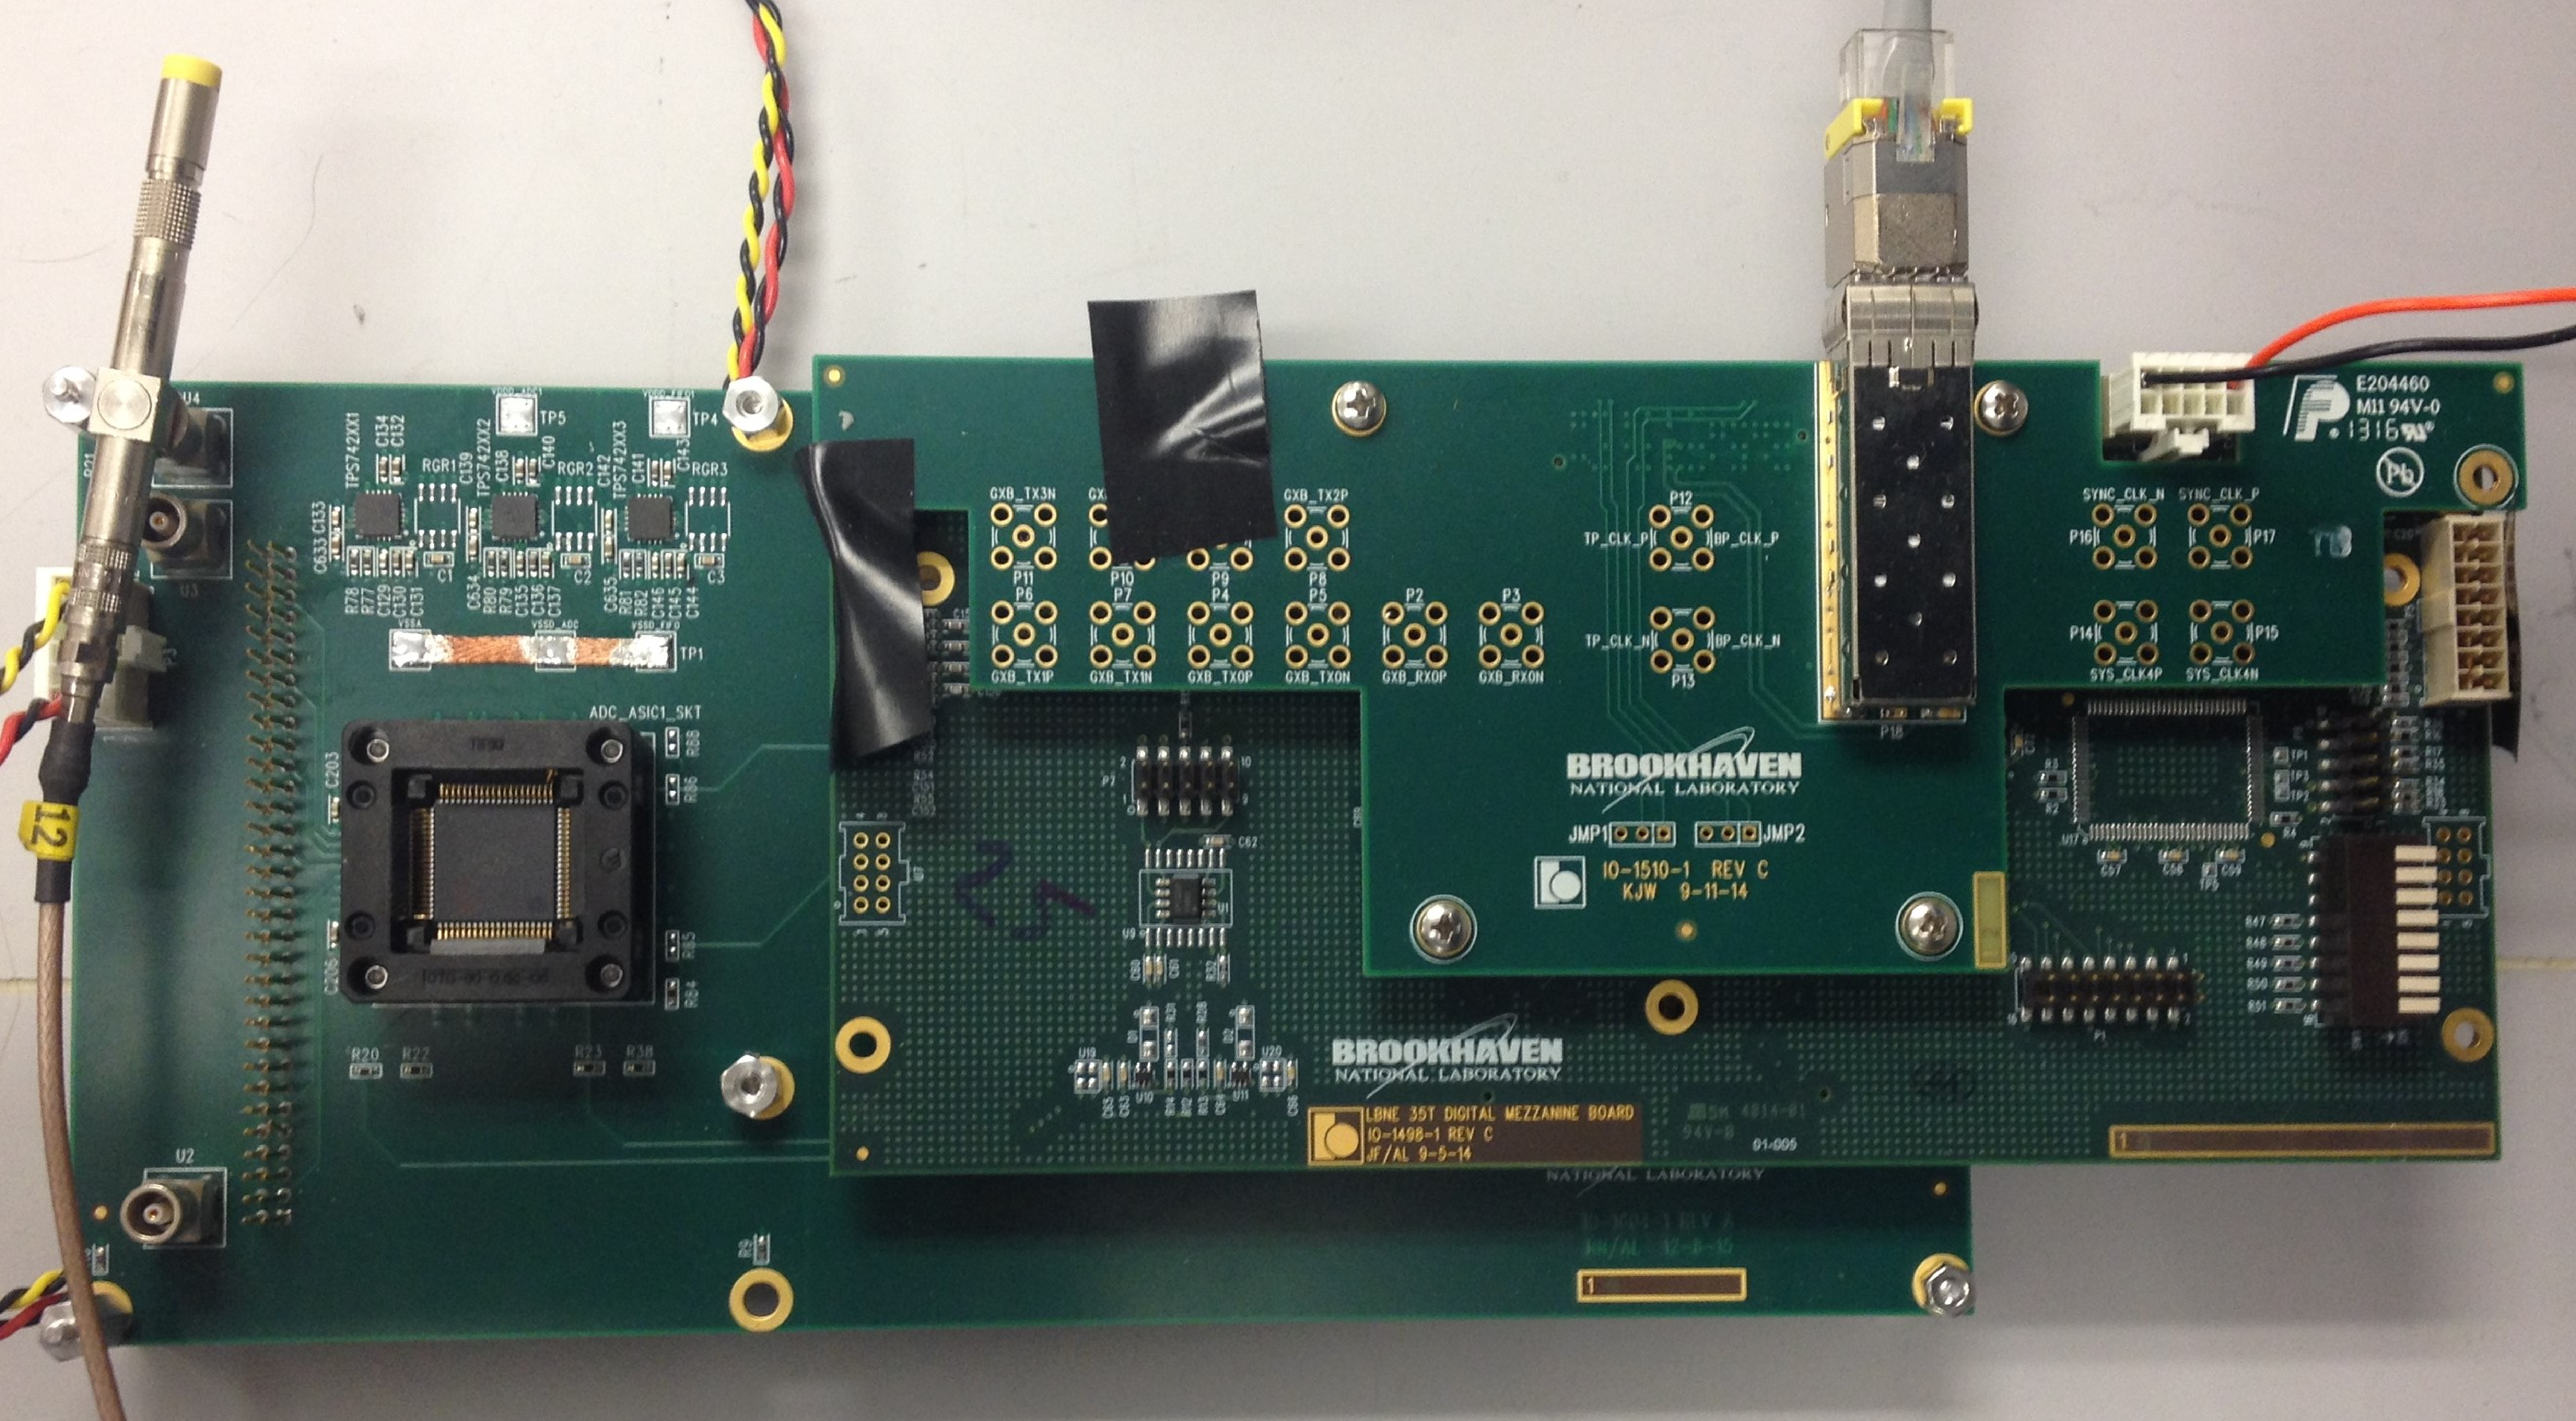
\includegraphics[width=0.6\linewidth]{tpcce_ADC_TestBoard.pdf}
\end{cdrfigure}

The development of the FE and ADC ASICs has proceeded through a series of prototype designs.
A 128-channel prototype analog mother board has been developed and tested in the lab.
Together with an FPGA mezzanine in place of the digital ASIC mezzanine,
they form a FEMB for use in the protoDUNE TPC,
since the COLDATA work is unlikely to be advanced enough to
provide more than a fraction of the electronics needed for the aggressive protoDUNE schedule.
A test stand has been developed to test the FEMB
using a commercial FPGA evaluation board as a mini-DAQ system.
All evaluation test data are stored on a desktop PC and analyzed to
determine whether the board is ready to be installed on the detector.

During the prototype testing, a procedure has been developed for the production test of the cold electronics boards.
This includes key parameters (gain, noise, non-linearity, etc.) that should be tested,
detailed steps of the test to collect data and extract these parameters,
and also the work flows to perform the test at both 300~K and 77~K.

Prototype cold electronics has been tested with prototype TPC and DAQ system,
to evaluate the performance of the APA assembly, and help the development of the DAQ software.
A vertical slice test has been used as the test bed for the integration test.
It is an important step to identify potential issues, check out system integration and performance
before the installation into the cryostat.

%%%%%%%%%%%%%%%%
\subsection{CE assembly testing}
\label{subsubsec:ce_install_assembly}

The front-end readout boards will be thoroughly tested. A testing program has been identified:
\begin{itemize}
\item A small number of the ASICs will undergo a complete suite 
of tests, including thermal cycling to determine the batch yield.
\item If the yield is high ($>$ 95\%), all ASICs will be mounted 
on the front-end boards.
Tests will be performed on each board and bad chips replaced as needed.
\item If the yield is not high, an automated test fixture will be 
fabricated to validate every ASIC chip before mounting on the readout boards.
Board-level tests after mounting the ASICs will be conducted.
However, previous experience indicates that this scenario is very unlikely.
\item The fully assembled front-end boards will be thermally cycled multiple times while connected
to a simple DAQ system to ensure reliable operation.
\item After the front-end electronics boards have been installed on an APA,
an initial calibration of all electronic channels will be performed.
The electronic gains and noise levels of all channels will be recorded in a database.
\item Electronic calibration on all channels will be performed while the APA is cold and again after it is warmed up.
\end{itemize}

%%%%%%%%%%%%%%%%%%%%%%%%%
\section{Beam plug}

As a part of the QC process for the beam plug, the vendor will conduct the following acceptance tests for the production units before shipping:
\begin{itemize}
\item {Initial helium leak check}
\item {Internal pressure check at cryogenic temperature (at about 2x operating pressure)}
\item {Post-test helium leak check to assess potential damage}
\item {External pressure check at room temperature (below 100 psi)}
\item {Final helium leak check to ensure no damage has been incurred}
\end{itemize}
The acceptable leak rate is below 15.6$\times 10^{-5}$ scc/s (He gas equivalent).
The tests performed by the vendor are primarily related to pressure safety and leak rates. Some of those tests will be repeated by LBNL upon receiving the units to verify vendor's results. In addition, LBNL will conduct tests to verify other aspects of the beam plug, in particular, the HV characteristics. The HV tests will be conducted using various facilities as described in the following sections.

\paragraph{BLANCHE Test Stand}
The BLANCHE test stand at Fermilab is a LAr cryostat dedicated to study high voltage related issues. It is 152 cm tall with a 76 cm inner diameter. The test stand is connected to a LAr purification system to remove oxygen and water contamination. The test stand is capable of delivering up to 150 kV to the sample. The cryostat is large enough to test a full size beam plug. The plan is to test the beam plug in BLANCHE to verify that the beam plug can withstand HV in LAr environment.
\\fixme{earlier nominal value across beam plug was said to be 165kV - so, test is not covering full range. Maybe add sentence to address this issue.}

\paragraph{Test in Charged Particle Beam}
During ProtoDUNE-SP physics runs, a charged particle beam will go through the beam plug with a rate of up to 100 Hz during a beam spill. The current induced from the ionization of the nitrogen gas by the charged beam particles is expected to be small; less than 1 nA during the spill. Given the low ionization rate and long pause between spills, we do not expect the charged particle beam to introduce electrical breakdown inside the beam plug. However, we plan to verify the design by putting the beam plug in a test beam with the beam plug at nominal HV. We will study the current flow inside the beam plug as a function of beam rate and nitrogen gas pressure. To minimize possible HV breakdown on the outer surface of the beam plug, which may complicate the interpretation of the test results, the beam plug will be immersed in dielectric oil. The test apparatus with the beam plug installed inside the setup is shown in Figure~\ref{fig:beamwindow_SLAC}.
\begin{cdrfigure}[SLAC beam test]{beamwindow_SLAC}{Beamplug test setup in electron beam to test electrical breakdown in the N filler gas.}
  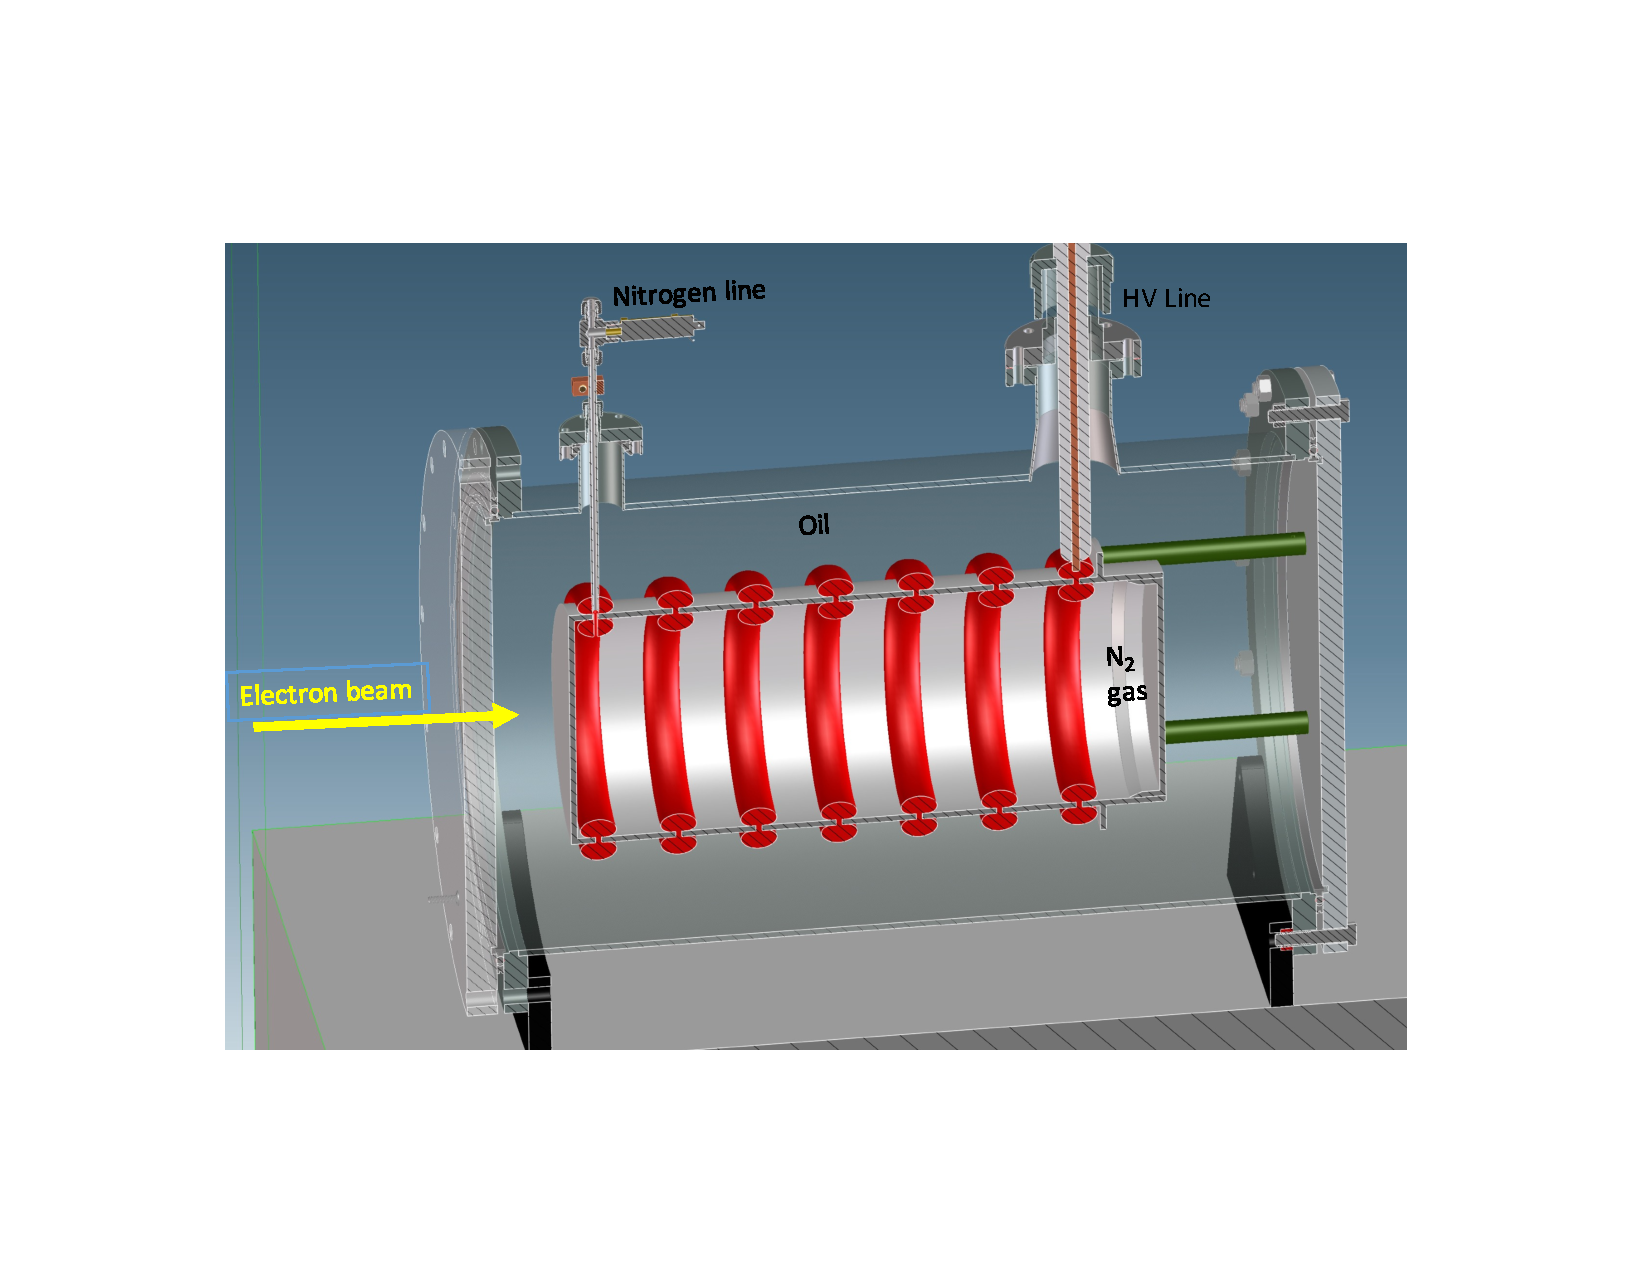
\includegraphics[width=0.6\textwidth]{beamwindow_SLACtest.pdf}
\end{cdrfigure}

\paragraph{Full integration test in 35-ton cryostat}
The final QC test of the beam plug is conducted inside the 35-ton cryostat at Fermilab. A small field cage mock-up is constructed and assembled inside the cryostat along with the beam plug. For this test, the beam plug is mounted to the field cage using a mounting scheme which is identical to the ProtoDUNE-SP one. The field cage mock-up will only have the first 10 profiles of a TPC, however, they will be operating at the nominal voltages. Therefore, the planned test will be a full-field test with the beam plug integrated into the field cage and the rest of the HV systems. A successful test would entail operating the TPC at the nominal HV (CPA at -180 kV) with the beam plug attached and that the electrical performance of the field cage with and without the beam plug is functionally the same.

\begin{cdrfigure}[PC4 Test setup]{beamwindow_PC4}{Field cage mock-up high voltage test in 35-ton cryostat \fixme{preliminary drawing}.}
  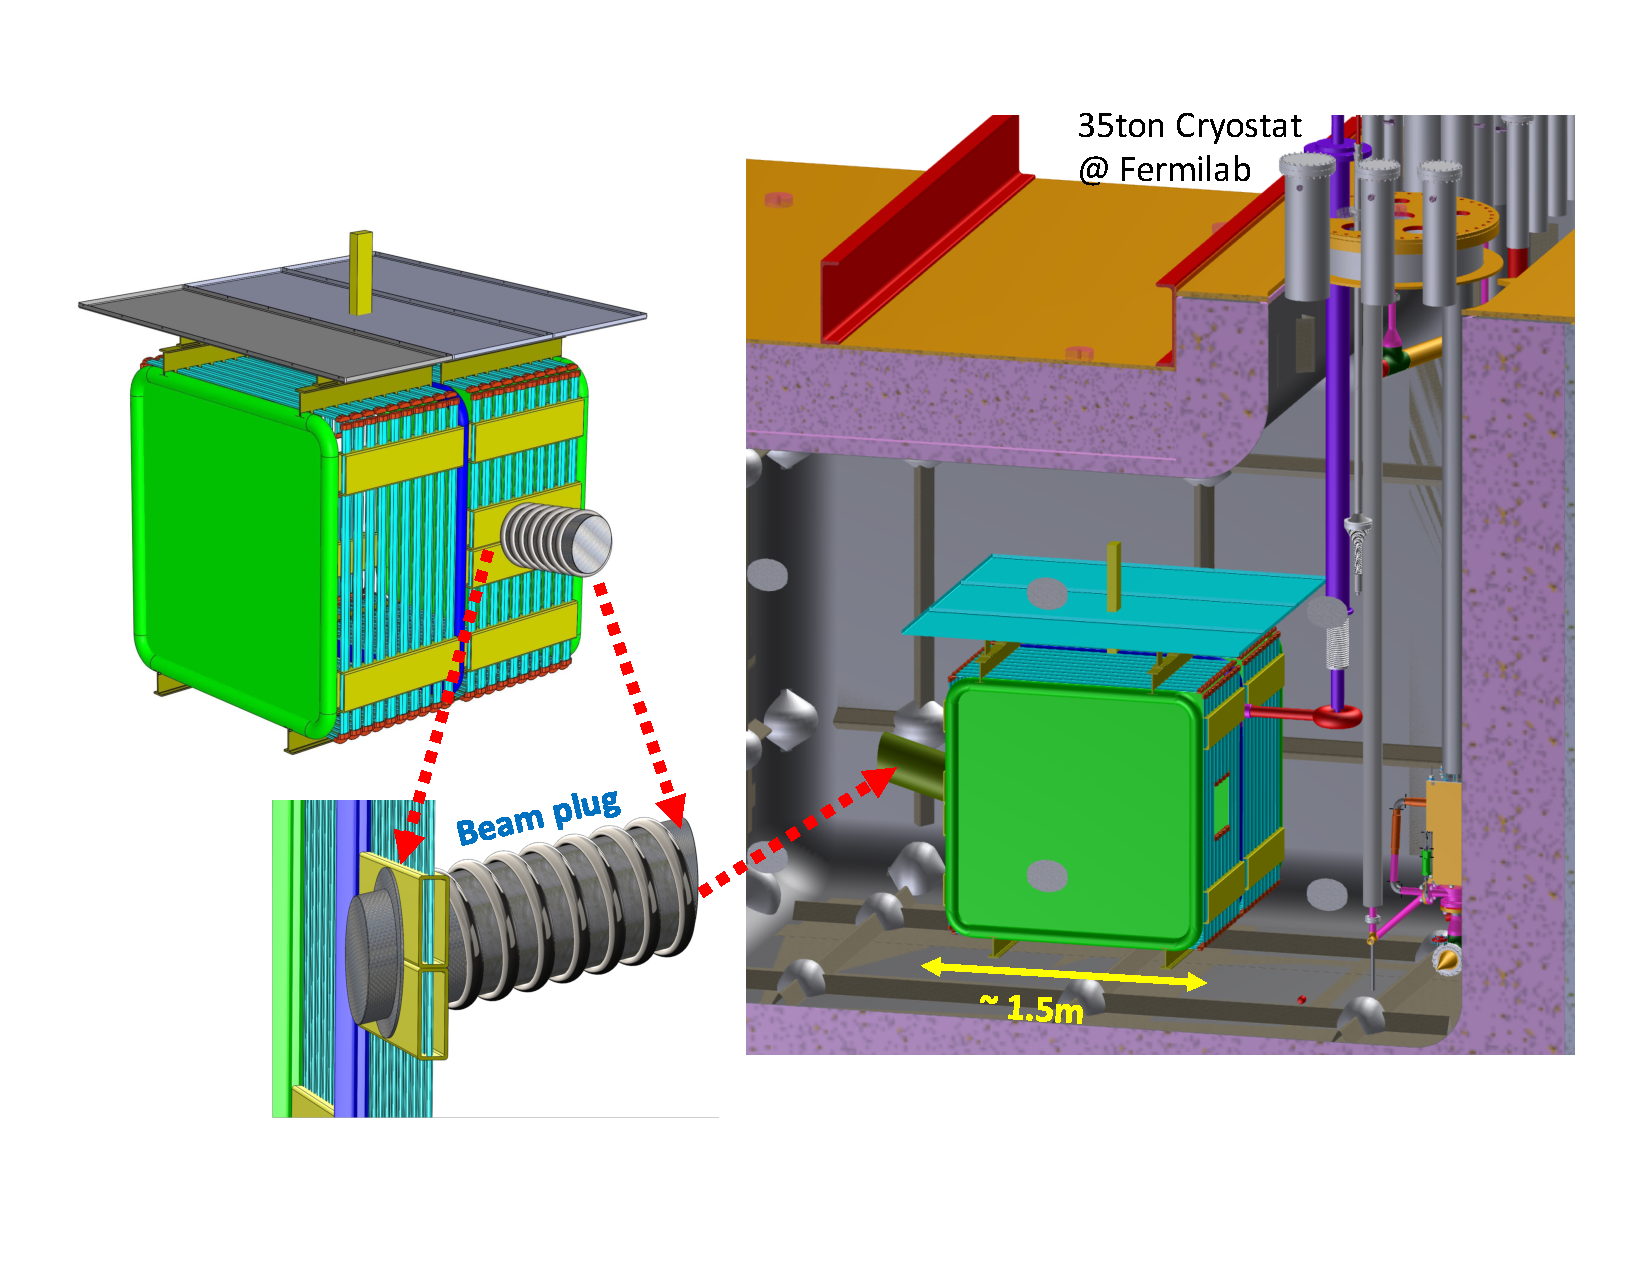
\includegraphics[width=0.95\textwidth]{beamwindow_PC4Test.pdf}
\end{cdrfigure}



